\chapter{Cost-sensitive logistic regression}\label{ch:7}

\begin{remark}{Outline}
In this chapter, we present a new cost-sensitive logisitic regression. The model consists in a new
logistic regression cost function, one that takes into account the real costs due to 
misclassification and correct classification. First, in Section \ref{sec:7:logistic}, we give the 
background behind logisitic regression. Then, in Section \ref{sec:7:cslr}, we described our 
previously proposed cost-sensitive logistic regression. For this, we do a deep analysis of the 
logistic regression implicit misclassification costs in Section \ref{sec:7:log_cost_analysis}. Then 
in Section \ref{sec:7:cscostfunction}, we shown a new version of the logistic regression cost 
function, one that takes into account the real costs due to misclassification and correct 
classification. Afterwards, in Section \ref{sec:7:ga}, we give a brief introduction to genetic 
algorithms, since is the model used to estimate the parameters of our proposed cost-sensitive 
logistic regression. Finally, in Section \ref{sec:7:results}, we compare the results of the proposed 
algorithm, against state-of-the-art methods, using the five real-world cost-sensitive databases.
\end{remark}


\section{Logistic regression}
\label{sec:7:logistic}

Logistic regression is a classification model that, in the specific context of binary 
classification, estimates the posterior probability of the positive class, as the logistic sigmoid 
of a linear function of the feature vector \citep{Bishop2006}. The estimated probability  is 
evaluated as 
\begin{equation}
  \hat p_i = P(y=1 \vert \mathbf{x}_i) = h_{\theta}(\mathbf{x}_i) = 
  g\bigg(\sum_{j=1}^{k}{\theta^jx_i^j}\bigg),
\end{equation}
where $h_\theta(\mathbf{x}_i)$ refers to the hypothesis of $i$ given the parameters $\theta$,  
and  $g(\cdot)$ is the logistic sigmoid function, defined as
\begin{equation}
  g(z)=\frac{1}{(1+e^{-z})} 
\end{equation}
In the next Figure, the logistic sigmoid function is shown.
\begin{figure}[htbp]
  \centering
  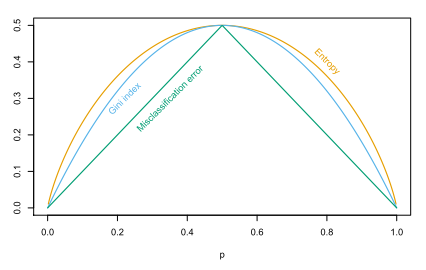
\includegraphics{ch7_fig1}
  \caption{Sigmoid function}
  \label{fig:ch7:1}
\end{figure}

The problem then becomes on finding the right parameters that minimize a given cost function.   
Usually, in the case of logistic regression the cost function $J(\theta)$ refers to the negative   
logarithm of the likelihood, such that
\begin{equation}
  J(\theta)=\frac{1}{N}\sum_{i=1}^{N} J_i(\theta),
\end{equation}
where
\begin{align}\label{eq:7:lrcost}
  J_i(\theta) =  -y_i\log(h_\theta(\mathbf{x}_i)) -(1-y_i)\log(1-h_\theta(\mathbf{x}_i)).
\end{align}
Therefore, the parameters are found using the following equation
\begin{align}
  \theta = \argmin_\theta J(\theta).
\end{align}

\begin{remark}{Logistic regression estimation}
There are several methods used to estimate the logistic regression, in particular, maximum 
likelihood \citep{Hastie2009}, Newton, coordinate descent \citep{Murphy2012} and dual coordinate 
descent \citep{Yu2011}. Nevertheless, all these methods rely on the assumption of convexity of the
negative logarithm of the likelihood function. In the next section we analyze the convexity of the 
logistic regression.
\end{remark}

\subsection{Convexity analysis}

A function $f(\mathbf{x})$ which is twice-differentiable is convex if and only if its hessian 
matrix (matrix of second-order partial derivatives) is positive semi-definite \citep{Boyd2010}.
Therefore, with the objective of evaluating the convexity of the logistic function, first the first 
order partial derivatives are calculated as follows:

\begin{equation}
\left[ \begin{array}{c}
  \frac{\partial J(\theta)}{\partial \theta_1} \\[0.1in]	
  \frac{\partial J(\theta)}{\partial \theta_2} \\[0.1in]	
  \ldots \\[0.1in]	
  \frac{\partial J(\theta)}{\partial \theta_k}
\end{array} \right] =
\left[ \begin{array}{c}
  \frac{1}{N}\sum_{i=1}^{N}\left[x_i^{(1)}\left(h_\theta(\mathbf{x}_i)-y_i\right)\right]\\[0.1in]
  \frac{1}{N}\sum_{i=1}^{N}\left[x_i^{(2)}\left(h_\theta(\mathbf{x}_i)-y_i\right)\right]\\[0.1in]
  \ldots \\[0.1in]	
  \frac{1}{N}\sum_{i=1}^{N}\left[x_i^{(k)}\left(h_\theta(\mathbf{x}_i)-y_i\right)\right]\\[0.1in]	
\end{array} \right]
\end{equation}

Then, using the first order partial derivatives, the Hessian ($H$) can be generalized as
\begin{equation}
  \partialb{j1}{j2}=\frac{1}{N}\sum_{i=1}^{N}
  \left[\bigg(1-h_\theta(\mathbf{x}_i)\bigg)h_\theta(\mathbf{x}_i)x_i^{(j1)}x_i^{(j2)}\right],
\end{equation}
where, $j1$ and $j2$ $\in \{1\cdots k\}$. Which is the same as
\begin{equation}
H=\left[ \begin{array}{cccc}
  \partialb{1}{1} & \partialb{1}{2} & \cdots & \partialb{1}{k} \\[0.1in]  
  \partialb{2}{1} & \partialb{2}{2} & \cdots & \partialb{2}{k} \\[0.1in]  
  \cdots & \cdots & \cdots & \cdots \\[0.1in]  
  \partialb{k}{1} & \partialb{k}{2} & \cdots & \partialb{k}{k}  
\end{array} \right]
\end{equation}

For the cost function to be convex the Hessian matrix	must be positive-semidefinite, and
a function is positive-semidefinite if:  
\begin{equation}
  z^T\left[\nabla_x^2f(x)\right]z \ge 0 \quad  \forall z
\end{equation}
Applied to J($\theta$), it is necessary to proof
\begin{equation}\label{eq:7:pos1}
  z^T\left[H \right]z \ge 0 \quad  \forall z
\end{equation}
Moreover, $H$ can be rewritten, using only the internal part of the sum, since it do not 
dependent on $\theta$
\begin{equation}
 H = \frac{1}{N}\sum_{i=1}^{N} \left[ 
\bigg(1-h_\theta(\mathbf{x}_i)\bigg)h_\theta(\mathbf{x}_i)\mathbf{x}_i^T \mathbf{x} \right]. 
\end{equation}
Then, (\ref{eq:7:pos1}) becomes
\begin{align}
  z^T \left[\bigg(1-h_\theta(\mathbf{x}_i)\bigg)h_\theta(\mathbf{x}_i)\mathbf{x}_i^T 
\mathbf{x}\right] z,
\end{align}
which can be rewritten as
\begin{align}
  (1-h_\theta(\mathbf{x}_i))h_\theta(\mathbf{x}_i)\left(\mathbf{x}_i^Tz\right)^2 \ge 0.
\end{align}
Therefore, proving that $J(\theta)$ is convex, as $\left(\mathbf{x}_i^Tz\right)^2 
\ge 0$ and \\ $\left((1-h_\theta(\mathbf{x}_i))h_\theta(\mathbf{x}_i)\right)\ge 0$ because $0\ge 
h_\theta(\mathbf{x}_i) \ge 1$.


\section{Cost-sensitive logistic regression}
\label{sec:7:cslr}

In this section we introduce our proposed cost-sensitive logistic regression 
\citep{CorreaBahnsen2014b}. First, we motive the need to modify the logistic regression, as we 
analyze the implicit costs that the logistic regression assign to each misclassification error 
during the estimation of the parameters $\theta$. Then, we show our proposed algorithm.


\subsection{Analysis of the logistic cost function}
\label{sec:7:log_cost_analysis}

The logistic regression cost function, as described in (\ref{eq:7:lrcost}), implicitly assume that 
a false positives and a false negatives have the same cost, i.e. $C_{{FP}_i} = C_{{FN}_i}$ $\forall 
i \in \{1,\cdots,N\}$. This can be easily shown by analyzing the logistic cost function for both 
values of $y_i$ and the algorithm prediction $h_\theta(\mathbf{x}_i))$:

\begin{itemize}
\item If $y_i=0$ and $h_\theta(\mathbf{x}_i)) \approx 0$, 
\begin{align*}
 J_i(\theta) &= -y_i\log(h_\theta(\mathbf{x}_i)) -(1-y_i)\log(1-h_\theta(\mathbf{x}_i)) \nonumber \\
 &\approx -(0)\log((0)) -(1-(0))\log(1-(0)) \nonumber \\
 &\approx 0.
\end{align*}

\item If $y_i=0$ and $h_\theta(\mathbf{x}_i)) \approx 1$, 
\begin{align*}
 J_i(\theta) &\approx -(0)\log((1)) -(1-(0))\log(1-(1)) \nonumber \\
 &\approx \infty.
\end{align*}

\item If $y_i=1$ and $h_\theta(\mathbf{x}_i)) \approx 0$, 
\begin{align*}
 J_i(\theta) &\approx -(1)\log((0)) -(1-(1))\log(1-(0)) \nonumber \\
 &\approx \infty.
\end{align*}

\item If $y_i=1$ and $h_\theta(\mathbf{x}_i)) \approx 1$, 
\begin{align*}
 J_i(\theta) &\approx -(1)\log((1)) -(1-(1))\log(1-(1)) \nonumber \\
 &\approx 0.
\end{align*}
\end{itemize}

\noindent Then, we collect the previous results in a cost matrix:
  \begin{table}[htbp]
    \centering
    \footnotesize
    \begin{tabular}{c|c|c}
      \multicolumn{3}{c}{}\\
      \multicolumn{1}{c|}{}  & Actual Positive& Actual Negative \\
      \multicolumn{1}{c|}{} & $y=1$& $y=0$ \\
      \hline
      Predicted Positive    & \multirow{ 2}{*}{$C_{{TP}_i}\approx 0$} & 
      \multirow{2}{*}{$C_{{FP}_i}\approx \infty$} \\
      $c=1$ & &\\
      \hline
      Predicted Negative    & \multirow{ 2}{*}{$C_{{FN}_i}\approx \infty$} & \multirow{ 
      2}{*}{$C_{{TN}_i}\approx 0$} \\
      $c=0$ & &\\
    \end{tabular}
    \caption{Logistic regression cost matrix}
    \label{tab:2:1}
  \end{table} 
  
This confirm our notion that the logistic regression cost function implicitly assume that 
a false positives and a false negatives have the same cost. However, as discussed in previous 
chapters, this is not the case in several real-world applications.

  
\subsection{Cost-sensitive cost function}
\label{sec:7:cscostfunction}

In order to incorporate the different real costs, as showed in 
\tablename{~\ref{tab:3:cost_matrix}}, into the logistic regression. We start by analyzing the 
expected costs that a modified logistic regression cost function should made for each 
misclassification and correct classification case.
\begin{equation*}
  J^c_i(\theta) = 
  \begin{cases}
    C_{TP_i}    & \text{if} \phantom{-}  y_i = 1 \text{ and } h_\theta(\mathbf{x}_i) \approx 1  \\
    C_{TN_i}    & \text{if} \phantom{-}  y_i = 0 \text{ and } h_\theta(\mathbf{x}_i) \approx 0  \\
    C_{FP_i}    & \text{if} \phantom{-}  y_i = 0 \text{ and } h_\theta(\mathbf{x}_i) \approx 1  \\
    C_{FN_i}    & \text{if} \phantom{-}  y_i = 1 \text{ and } h_\theta(\mathbf{x}_i) \approx 0 .
  \end{cases}
\end{equation*}

Then, as we already have the real costs, we create a new cost-sensitive logistic regression cost 
function, by including the different costs into the logistic function,
\begin{align}\label{eq:CSLR}
  J^c(\theta)=\frac{1}{N} \sum_{i=1}^{N} \bigg( y_i(h_\theta(\mathbf{x}_i) C_{TP_i} + 
  (1-h_\theta(\mathbf{x}_i))C_{FN_i})  \nonumber\\ 
  +(1-y_i)(h_\theta(\mathbf{x}_i) C_{FP_i} + (1-h_\theta(\mathbf{x}_i))C_{TN_i}) \bigg).
\end{align}

Nevertheless, our previous analysis have shown that this new cost function is not always convex 
\citep{CorreaBahnsen2014b}, therefore, we estimate the parameters $\theta$ with genetic algorithms, 
as this optimization heuristic does not require the underlying function to be differentiable or 
convex \citep{Haupt2004}. In the next section we give a brief introduction to generic algorithms.


\subsection{Genetic algorithms}
\label{sec:7:ga}
\todo{DELETE??}

Genetic algorithms, is an optimization technique that attempts to replicate natural evolution 
processes in which the individuals with the considered best characteristics to adapt to the 
environment are more likely to reproduce and survive. These advantageous individuals mate between 
them, producing descendants similarly characterized, so favorable characteristics are preserved and 
unfavorable ones destroyed, leading to the progressive evolution of the species. The model aims 
to improve the solution to a problem by keeping the best combination of input variables. The 
flow diagram presented in \figurename{~\ref{fig:7:geneticalgorithms}} describes the process. It 
starts with the definition of the problem to optimize, generating an objective function to evaluate 
the possible candidate solutions (chromosomes), i.e., the objective function is the way of 
determining which individual produces the best outcome. 

The next step is to generate an initial random population of n individuals called chromosomes that 
are symbolized by binary strings, where each binary position of the chromosome is called a gene and 
denotes a specific characteristic (input variable). Therefore the combination of all the different 
characteristics encoded in the string represents an individual who is a candidate for the solution.
Each chromosome is evaluated in the objective function and the best individuals are selected to 
survive for mating (parents), while the worse ones are discarded to make room for new descendants.  
There are many ways of pairing the selected chromosomes \citep{Haupt2004}. In this paper, a 
weighted 
cost pairing is used, which consists of assigning a selection probability according to each 
chromosome cost. That is, a chromosome with the higher cost has a greater probability of mating 
because cost maximization is desired.

\begin{figure}[t]
  \centering
  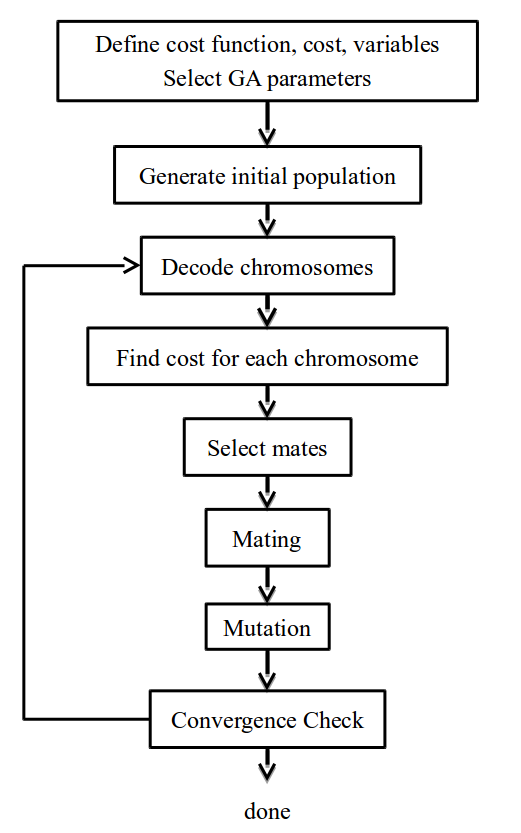
\includegraphics[width=8cm]{ch7_fig2}  
  \caption{Genetic algorithms \citep{Haupt2004}}
  \label{fig:7:geneticalgorithms}
\end{figure}
  
After selecting the parent chromosomes with the chosen pairing method, the next step is to create a 
second generation of individuals, based on the information of the parents. There are several ways 
of 
mating. In this paper, two parents create one child. 
In order to transfer the parents binary information to the child, there are also different kinds 
of approaches such as the one-point crossover. The one-point crossover technique consists in 
selecting one random point on the parents string. The child is created in the following way: First, 
the parent1 transfers its binary code from the first gene to the crossover point. Then the parent2 
transfers its binary code from the crossover point to the last gene of the chromosome. New parents 
are randomly selected for each new child and the process continues until the chromosome population 
grows back to the original size n. 

Once the breeding process is completed, random mutation is used to alter a certain percentage of 
the 
genes of the chromosomes. The purpose of mutation is to introduce diversity into the population, 
allowing the algorithm to avoid local minima by generating new gene combinations in the 
chromosomes. 
The most common mutation procedure is the one called single point mutation. It is implemented by 
generating a random variable that indicates the position of the gene that will be modified, from 
the 
population of chromosomes. Generally, mutation is not allowed in the best solution chromosomes 
because these elite individuals are destined to propagate unchanged. In genetic algorithm this 
is called elitism.

Finally, after mutation is done the new generation of chromosomes is evaluated with the objective 
function and used in the next iteration of the described algorithm.
The algorithm iterates until a maximum number of chromosome generations are created or a 
satisfactory solution is reached.


\section{Experiments}
\label{sec:7:results}
\todo{Experiments}


\begin{table}
    \centering
    \footnotesize
    \begin{tabular}{l l r@{\hskip 0in}c@{\hskip 0in}l r@{\hskip 0in}c@{\hskip 0in}l r@{\hskip 
    0in}c@{\hskip 0in}l  } %sum 7.7
    \hline
    \bf{Family} & \bf{Algorithm} & \multicolumn{3}{c}{\bf{Fraud}} & 
    \multicolumn{3}{c}{\bf{Churn}} & \multicolumn{3}{c}{\bf{Credit 1}} \\ 
    \hline
CI&LR-t & 0.0092 &$\pm$& 0.0002 & -0.0001 &$\pm$& 0.0002 & 0.0177 &$\pm$& 0.0126\\ 
&LR-u & 0.1243 &$\pm$& 0.0387 & 0.0039 &$\pm$& 0.0492 & 0.4118 &$\pm$& 0.0313\\ 
\hline 
CPS&LR-r & 0.3077 &$\pm$& 0.0301 & 0.0484 &$\pm$& 0.0375 & 0.3965 &$\pm$& 0.0263\\ 
&LR-o & 0.2793 &$\pm$& 0.0185 & 0.0316 &$\pm$& 0.0228 & 0.3301 &$\pm$& 0.0109\\ 
\hline 
BMR&LR-t-BMR & 0.4552 &$\pm$& 0.0203 & 0.1082 &$\pm$& 0.0316 & 0.2189 &$\pm$& 0.0541\\ 
\hline 
CST&CSLR-t & \bf{0.6113} &\bf{$\pm$}& \bf{0.0262} & \bf{0.1118} &\bf{$\pm$}& \bf{0.0484} & 
\bf{0.4554} &\bf{$\pm$}& \bf{0.1039}\\ 
\hline
  \multicolumn{11}{c}{(those models with the highest savings are market as bold)}
  \end{tabular}
    \caption{Results of the algorithms measured by savings}
    \label{tab:7:results_savings}
  \end{table}
  
\begin{table}
    \centering
    \footnotesize
    \begin{tabular}{l l r@{\hskip 0in}c@{\hskip 0in}l r@{\hskip 0in}c@{\hskip 0in}l  } %sum 7.7
    \hline
    \bf{Family} & \bf{Algorithm} &  \multicolumn{3}{c}{\bf{Credit 2}} 
& \multicolumn{3}{c}{\bf{Marketing}} \\ 
    \hline
CI&LR-t & 0.0039 &$\pm$& 0.0012 & -0.2931 &$\pm$& 0.0602\\ 
&LR-u & 0.1850 &$\pm$& 0.0231 & 0.2200 &$\pm$& 0.0376\\ 
\hline 
CPS&LR-r & 0.2650 &$\pm$& 0.0115 & 0.4210 &$\pm$& 0.0267\\ 
&LR-o & 0.2554 &$\pm$& 0.0090 & 0.3129 &$\pm$& 0.0277\\ 
\hline 
BMR&LR-t-BMR & \bf{0.3148} &\bf{$\pm$}& \bf{0.0094} & \bf{0.4973} &\bf{$\pm$}& \bf{0.0084}\\ 
\hline 
CST&CSLR-t & 0.2748 &$\pm$& 0.0069 & 0.4484 &$\pm$& 0.0072\\ 
\hline 
  \multicolumn{8}{c}{(those models with the highest savings are market as bold)}
  \end{tabular}
    \caption{Continuation of \tablename{~\ref{tab:7:results_savings}}.}
    \label{tab:7:results_savings2}
  \end{table}

\begin{figure}[!t]
  \centering
  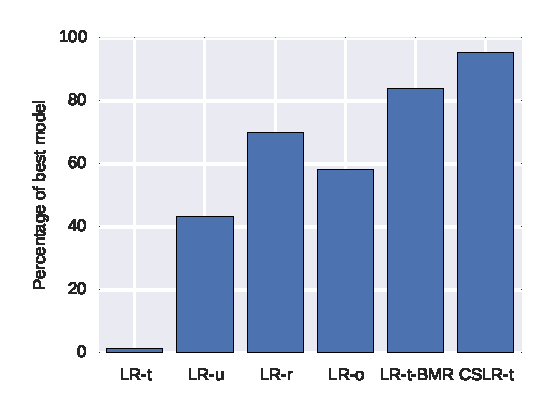
\includegraphics{ch7_fig3}
  \caption{\textbf{Comparison of the average savings of the algorithms versus the 
    highest savings.} When the probabilities are calibrated there is a 
    significant increase in savings.}
  \label{fig:7:comparison_per_best}
\end{figure}


\begin{figure}[!t]
  \centering
  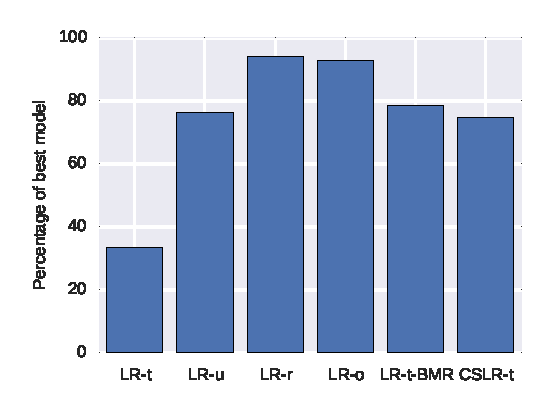
\includegraphics{ch7_fig4}
  \caption{\textbf{Comparison of the average savings of the algorithms versus the 
    highest savings.} When the probabilities are calibrated there is a 
    significant increase in savings.}
  \label{fig:7:comparison_per_best_fscore}
\end{figure}